\chapter{The World Bank's Data}\label{chap_data}

As shown on chapter \ref{chap_intro}, collecting the necessary data for any Data Science project is almost always a huge task because the reality tends to be that some of the most relevant variables commonly go unmeasured or are private. This project uses  two types of data, private and public. This chapter describes the two main types of data used for this project.
Section \ref{sec_inv_data} describes the characteristics of private data and the scope it has. It also explains about the confidentiality agreement Integrity Vice Presidency (INT) offered this project in exchange for investigations data. Section \ref{sec_public_data} explains how to download public data from the Wold Bank's servers using coding tools.

\section{Investigations data}\label{sec_inv_data}

The most valuable data for this project was the private data which the partners at INT made available for the project while maintaining a spirit of openness. A confidentiality agreement was signed in order to give access to the investigations database. The only condition was that all the data and analyses had to be stored and processed on a remote server with an encryption and security measurements that satisfied the World Bank's standards. 

In this case the server was an Amazon Web Service's (AWS), Amazon Elastic Compute Cloud (Amazon EC2) machine. EC2 is a web service that provides resizable compute capacity in the cloud. It is designed to make web scale cloud computing easier for developers\footnote{``Amazon EC2’s simple web service interface allows you to obtain and configure capacity with minimal friction. It provides you with complete control of your computing resources and lets you run on Amazon’s proven computing environment. Amazon EC2 reduces the time required to obtain and boot new server instances to minutes, allowing you to quickly scale capacity, both up and down, as your computing requirements change. Amazon EC2 changes the economics of computing by allowing you to pay only for capacity that you actually use. Amazon EC2 provides developers the tools to build failure resilient applications and isolate themselves from common failure scenarios.'' \parencite{aws_es2}}. For more details on how to setup an AWS computer see \parencite{aws_start} and appendix \ref{chap_software}. In other words, the data was stored in an AWS machine on the cloud that had an encrypted folder with the specific files. Since all the data had to stay on the cloud, all the processing had to be done on the cloud too. For this purpose, a server running \texttt{Python} and \texttt{R} was hosted at an AWS computer. 


\subsection{Basic description}

The investigations data consists of nearly 13,000 cases, of which over half are Fraud and Corruption. 377 are labeled as Collusion. These are from the ``Allegation Category'' column, Notably, allegation categories include Fraud, Corruption, and Fraud \& Corruption. It is possible for a case's description to just say Fraud and for its allegation category to still be Fraud and Corruption. I would suggest treating each of these 3 categories as the same (i.e. all ``Fraud and Corruption'').

Allegations also include a ``Allegation Sub-Category''. Collusion is sometimes listed as a sub-category, for example: Allegation Category: Fraud and Corruption or Allegation Sub-Category: Bid Manipulation/Collusion.

The Unit of analysis is the investigations data is the ``Subject'' column. Mostly this variable refers to companies and people, but on occasion other entities on a project may be subjects of investigation, for example the coordinating agency. For example Case \# C-EGT-2010-1754, the subject is: Egyptian Ministry of Education. In procurement data it shows up in ``Implementing Agency'' column as: \texttt{PPMU-MINISTRY OF EDUCATION}
    
The Labels in the investigations are very different and specific to each investigation case. The most relevant label will be the Allegation Outcome's column. The most frequent outcomes for a case are ``Substantiated'', which means that the Subject was found to be guilty of the Allegation, ``Unfounded'', which means that the Subject was found to be  innocent of the allegation, and ``Unsubstantiated'', which means that the investigation did not have the necessary means to conclude that the subject was  guilty, but neither does it have to conclude that the subject is innocent. Substantiated and Unsubstantiated occur in roughly equal quantities, while Unfounded is fairly rare. There are other, rarer labels, like ``We kicked it to another organization''.

The identities of the cases within the investigations data include that about 80\% of the data has either the name of the accused (the majority) or the project number (about a third). These are in the Subject and Project Number columns, respectively. That means about 20\% of the data appears to be ``lost'', in that we can't match it up to any procurement data. There is potentially other information in the ``Title'' field, but it is unstructured. There could theoretically be information in other fields, but they are not as rich.

There are among 1000 different sectors but most of them are mixed sectors and have not been previously cleaned. For example, when an investigation involves cases that cover sectors such as transportation and urban development there can be the case that you find a Transportation sector, a Urban Development sector and a Transportation \& Urban Development Sector. For the specifics of the model, this project works with sector specific as they are, this meaning that, for the project, the three cases mentioned before are considered to be different sectors. By doing so, there are about 205 sectors.

% Questions [for Betsy?]
% ==
% - What's the difference between 'Allegation Outcome' and 'Outcome of Overall Investigation When Closed', because these often give different outcomes (Substantiated, Unsubstantiated) (Outcomes different: 10422, Outcomes same: 2301)
% - In sector names, what's the difference between "Transportation" and "SDN - Transport"
%  - Ditto "Energy/Mining" and "SDN - Energy/Mining"





\section{Public data}\label{sec_public_data}


Fortunately for the project, not all the data was private. This work uses the Open Data\footnote{Go to \cite{wb_data}.}  and the Data Bank websites from the World Bank, which offer free access to comprehensive, downloadable indicators about development in countries around the globe. 

Public data from the World bank comes from different databases. They are generated at different sections within the World Bank so each indicator can be obtained form a specific database according to its nature. For example, all the Development indicators can be obtained at the World Bank's World Development Indicators database, indicators regarding how easy it ts to do business in each specific country could be obtained from the Doing Business database and indications regarding world's populations can be obtained at the Health Nutrition and Population Statistics database.\footnote{Different databases include:
Africa Development Indicators, Statistical Capacity Indicators, Country Policy and Institutional Assessment (CPIA), Country Partnership Strategy for India, Corporate Scorecard, Doing Business, Exporter Dynamics Database: Country-Year, Education Statistics, Enterprise Surveys, Global Findex ( Global Financial Inclusion database), G20 Basic Set of Financial Inclusion Indicators, Gender Statistics, Global Economic Monitor, GEP Economic Prospects, Global Financial Development, Global Economic Monitor (GEM) Commodities, Global Partnership for Education, Global Social Protection, Health Nutrition and Population Statistics, Health Nutrition and Population Statistics by Wealth Quintile, Health Nutrition and Population Statistics: Population estimates and projections, International Development Association - Results Measurement System, INDO-DAPOER, International Debt Statistics, Jobs for Knowledge Platform, LAC Equity Lab, Millennium Development Goals, Povstats, Quarterly Public Sector Debt, Quarterly External Debt Statistics/GDDS (New), Quarterly External Debt Statistics/SDDS (New), Readiness for Investment in Sustainable Energy (RISE), Sustainable Energy for All, Subnational Malnutrition Database, Subnational Poverty, Subnational Population, Wealth accounting, World Development Indicators and the  Worldwide Governance Indicators.}

A good practice in Data Science is to generate code so that all results can be easily replicated. That was the reason why, for this project all the data that the World Bank bank provides publicly by an Application Programming Interface (API) was collected with reliable code. Thanks to prior World Bank's work, accessing the World Bank Data APIs with code in languages such as \texttt{Python}, \texttt{R}, \texttt{Ruby} and \texttt{Stata} is a simple task. The World Bank has a blog where they explain in detail how to use the APIs. See the \cite{wb_api}, the \cite{wb_python} and the \cite{wb_r} for more details on how to do this. To put things in context, \texttt{Python} and \texttt{Ruby} are general-purpose programming languages, and \texttt{Stata} and \texttt{R} are programming environments optimized for statistics. They're all widely used in the business and academic worlds. The World Bank generates modules to those languages which help users to connect to the World Bank Development Indicators API and access the latest data.

For example, in \texttt{python}, the \texttt{wbdata} module by Oliver Sherouse offers easy access to all the data in the World Bank's APIs. It also plays nicely with Wes McKinney’s  \texttt{pandas} analysis library\footnote{See appendix \ref{chap_software} for \texttt{pandas} details.}. \texttt{Wbdata} is a simple python interface to find and request information from the World Bank's various databases, either as a dictionary containing full meta data or as a \texttt{pandas} Data Frame. Currently, \texttt{wbdata} wraps most of the World Bank API, and also adds some convenience functions for searching and retrieving information.

In \texttt{R}, the \texttt{WDI} module by Vincent Arel-Bundock offers convenient access to the data in the World Bank's API. For fast searching, the \texttt{WDI} package ships with a local list of available data series. This local list can be updated to the latest version using the \texttt{WDIcache} function \parencite{wb_r}. Similar tools are available to languages such as Ruby and Stata.

Given that, the public data used in this project can be divided in two sets; first, the World Bank's World Development Indicators, which can be obtained by using the API and the packages mentioned; and, second, all the historical and major awards given by the World Bank to all developing countries from 1990 to 2014. 


\subsection{World Development Indicators}

The World Bank has a major data base called: World Development Indicators (WDI). WDI is the primary World Bank collection of development indicators, compiled from officially recognized international sources. This database represents the most current and accurate global development data available, and includes national, regional and global estimates. For the purpose of this work, the indicators selected such that prediction of corruption, collusion and fraud would not be attainable to specific country variables such as country or country region. This is was because the World Bank can not start investigation cases in specific countries just because different countries tend to have different levels of corruption. Unfortunately, those types of variables can have, in some times, much better prediction rates but the policies at the World Bank prevents a model of having them for discretion and discrimination arguments.

Also, the World Bank has around 16,000 different indicators the project could use, but being this big, and according to purpose of this project, only a few indicators were selected. The next list shows the ones that were considered. This list includes indicators related to the private sector and trade among countries which is the theme the project is targeting.

\begin{description}
\item[IC.BUS.DISC.XQ]	Private Sector \& Trade: Business environment. Business extent of disclosure index (0=less disclosure to 10=more disclosure)	Disclosure index measures the extent to which investors are protected through disclosure of ownership and financial information. The index ranges from 0 to 10, with higher values indicating more disclosure.
\item[IC.FRM.CMPU.ZS]	Private Sector \& Trade: Business environment. Firms competing against unregistered firms (\% of firms).
\item[IC.FRM.CORR.ZS]	Private Sector \& Trade: Business environment	Informal payments to public officials (\% of firms).
\item[IC.FRM.INFM.ZS]	Private Sector \& Trade: Business environment	Firms that do not report all sales for tax purposes (\% of firms).
\item[IC.LGL.CRED.XQ]	Private Sector \& Trade: Business environment	Strength of legal rights index (0=weak to 10=strong).
\item[IC.LGL.DURS]	Private Sector \& Trade: Business environment	Time required to enforce a contract (days).
\item[IC.TAX.GIFT.ZS]	Private Sector \& Trade: Business environment	Firms expected to give gifts in meetings with tax officials (\% of firms).
\item[IQ.CPA.PROP.XQ]	Public Sector: Policy \& institutions	CPIA property rights and rule-based governance rating (1=low to 6=high).
\item[IQ.CPA.TRAN.XQ]	Public Sector: Policy \& institutions	CPIA transparency, accountability, and corruption in the public sector rating (1=low to 6=high).
\item[NY.GDP.PCAP.CD]	Economic Policy \& Debt: National accounts: USD at current prices: Aggregate indicators	GDP per capita (current US\$).
\item[SE.PRM.PRSL.ZS]	Education: Efficiency	Persistence to last grade of primary, total (\% of cohort).
\item[SI.POV.GINI]	Poverty: Income distribution GINI index.
\item[SL.UEM.TOTL.NE.ZS]	Social Protection \& Labor: Unemployment	Unemployment, total (\% of total labor force) (national estimate).
\end{description}

The code to download WDI can be seen at the Appendix \ref{chap_code} in code \ref{code_wdi}. This code can easily replicate results. For the purpose of this work, the code in \ref{code_wdi} downloads data for the countries within the countries from the investigations data, those countries define the countries list for this work.



\begin{figure}[H]
\begin{center}
\caption{WDI: \% of Bribes to tax officials per Country/Region}
\label{fig_wdi_bribes}
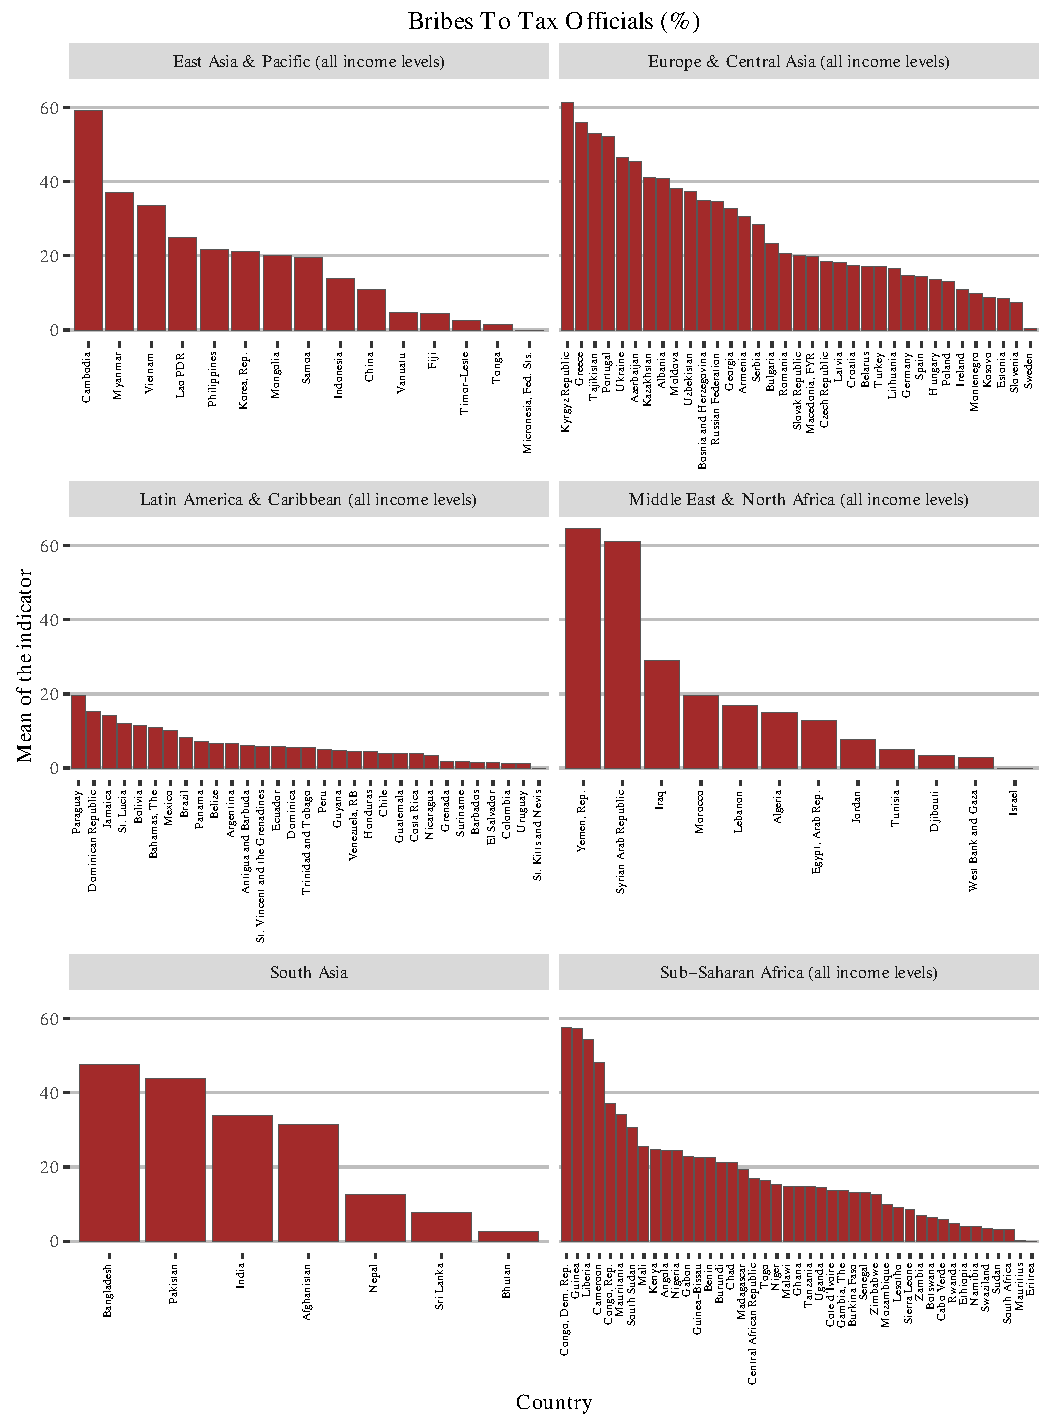
\includegraphics[max height=.9\textheight]{../img/wdi_bribes_to_tax_officials_perc.pdf}
\end{center}
\noindent \footnotesize{\textbf{Source:} Own creation and data obtained with package \texttt{WDI}, see the \cite{wb_r}.}
\end{figure}

\begin{figure}[H]
\begin{center}
\caption{WDI: \% of Firms competing against informal firms per country/Region}
\label{fig_wdi_firms}
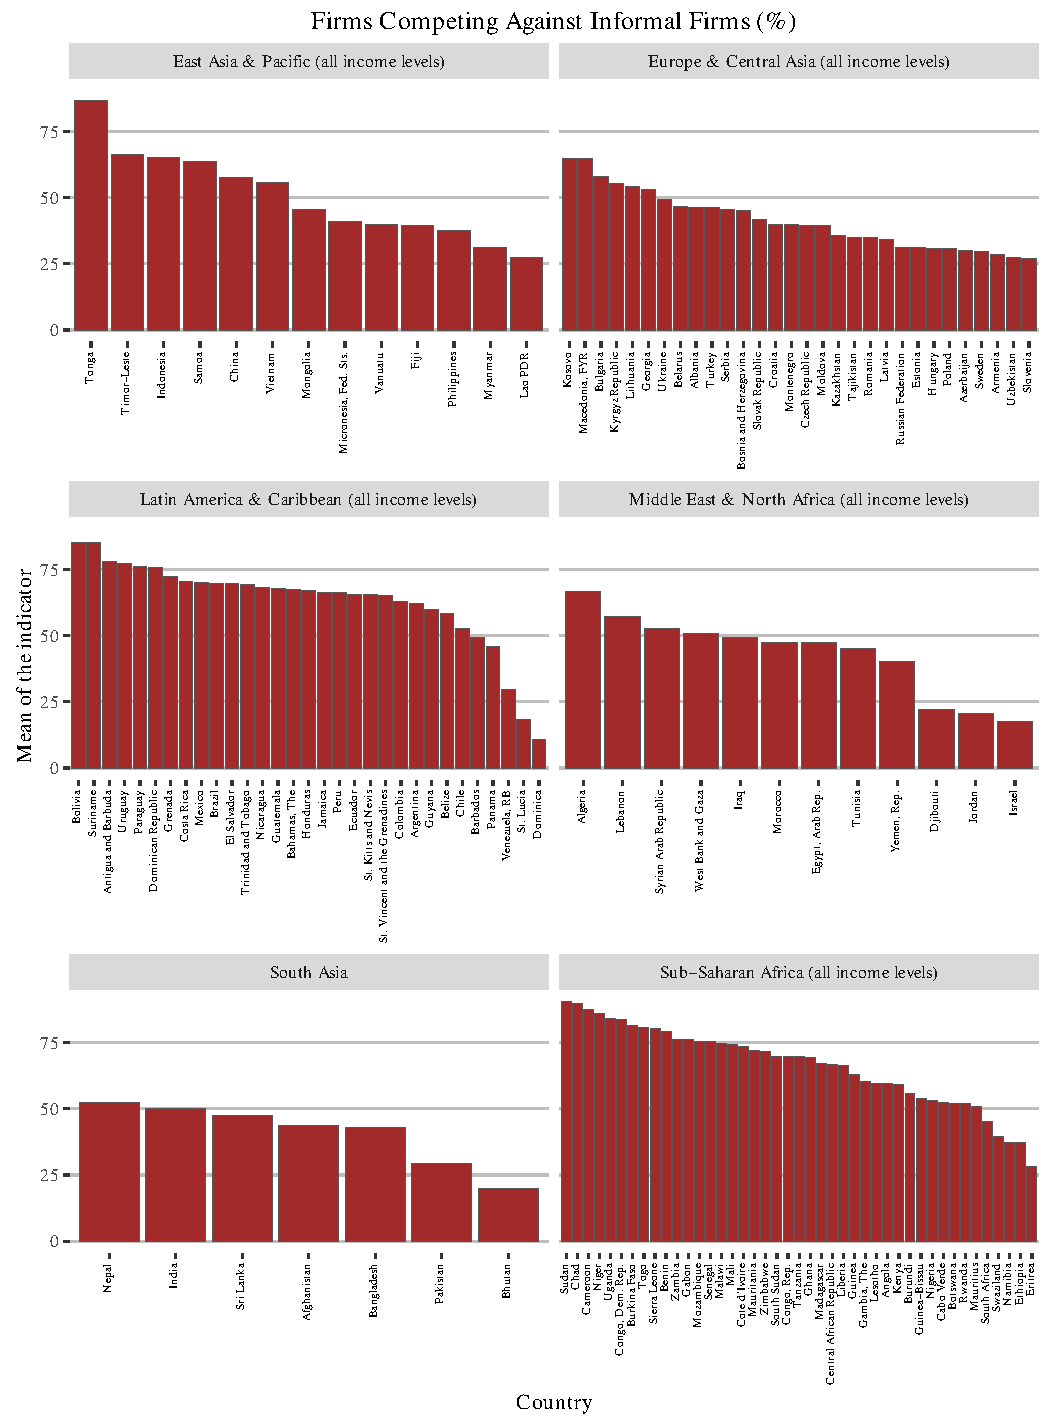
\includegraphics[max height=.9\textheight]{../img/wdi_firms_competing_against_informal_firms_perc.pdf}
\end{center}
\noindent \footnotesize{\textbf{Source:} Own creation and data obtained with package \texttt{WDI}, see the \cite{wb_r}.}
\end{figure}

\begin{figure}[H]
\begin{center}
\caption{WDI: \% of Payments to public officials per Country/Region}
\label{fig_wdi_pays}
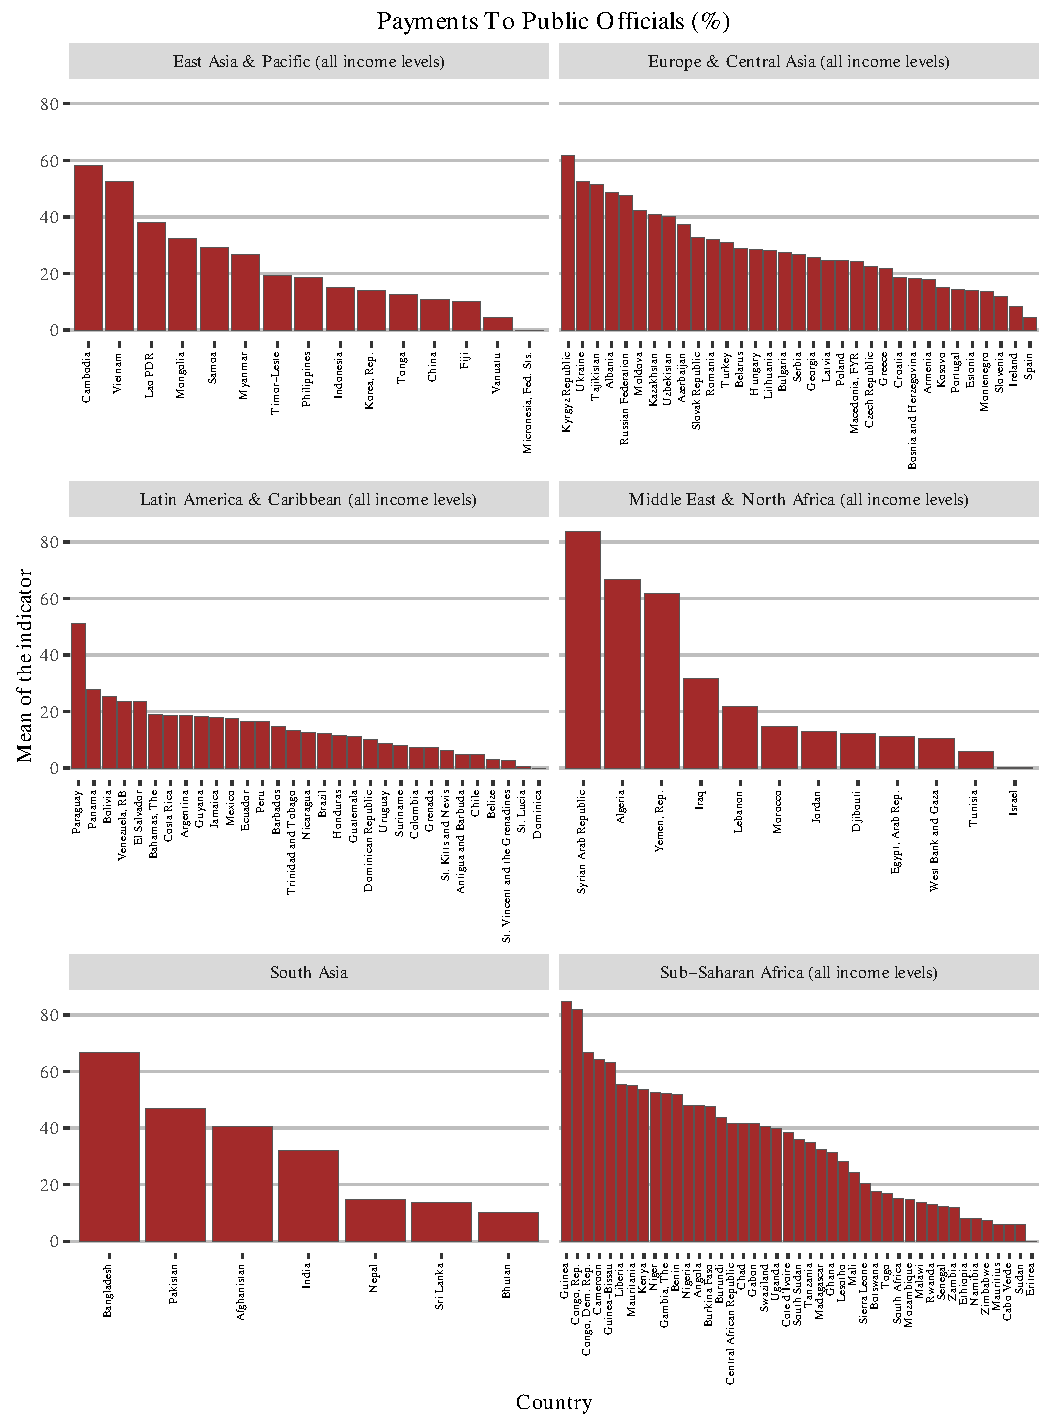
\includegraphics[max height=.9\textheight]{../img/wdi_payments_to_public_officials_perc.pdf}
\end{center}
\noindent \footnotesize{\textbf{Source:} Own creation and data obtained with package \texttt{WDI}, see the \cite{wb_r}.}
\end{figure}


\begin{figure}[H]
\begin{center}
\caption{WDI: Time to Enforce Contracts per Country/Region}
\label{fig_wdi_time_contract}
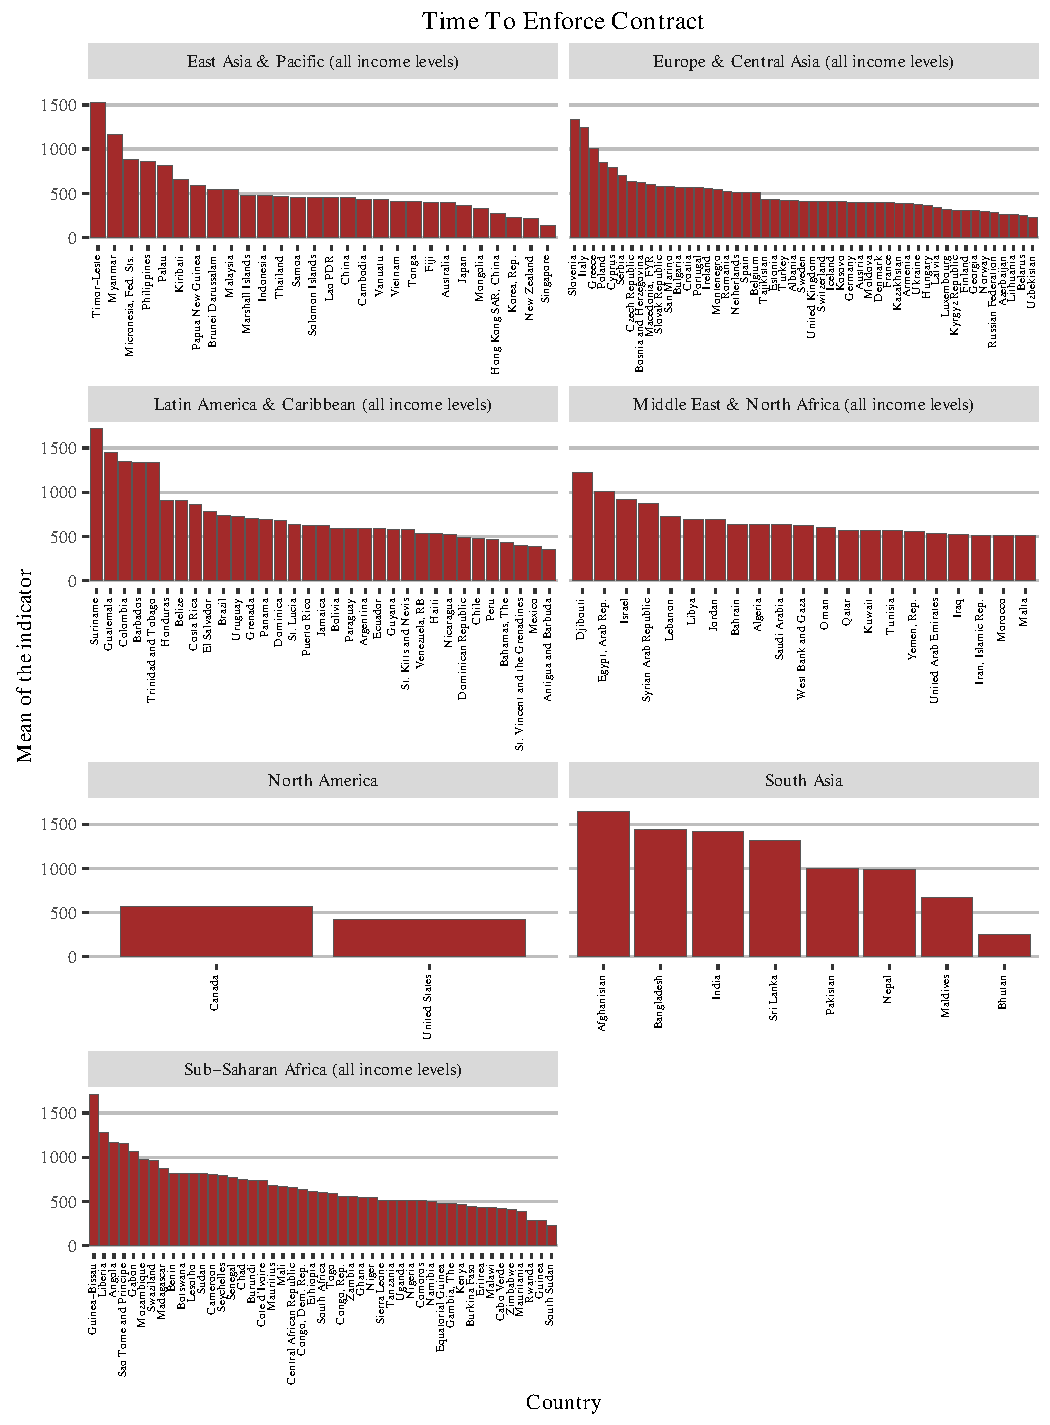
\includegraphics[max height=.9\textheight]{../img/wdi_time_to_enforce_contract.pdf}
\end{center}
\noindent \footnotesize{\textbf{Source:} Own creation and data obtained with package \texttt{WDI}, see the \cite{wb_r}.}
\end{figure}


\subsection{Major and Historic Awards}



\section{Disambiguation}